\long\def\comment#1{}

\comment{Our goal is to estimate the connection matrix from a population of observable neurons, given only their calcium fluorescence observations. We take a model based approach, meaning that we first describe a parametric generative model that completely characterizes the statistics of the data, and then we derive algorithms to learn the parameters, given the data.

We use the following conventions throughout the paper, unless indicated otherwise. Time is discrete, taking values $t=1,\ldots,T$. We let $X_i(t)$ indicate the state of neuron $i$ at time $t$, $X_i=\{X_i(t), t=1,\ldots, T\}$, and ${\bf X}= \{X_1, \ldots, X_N\}$. Conditional probability distributions will be written $P[\bf F | \bf X; \bth]$, where $\bf X$ indicates some random variables, $\bth$ indicates some parameters, and a semicolon separates the two. To indicate that a random variable, $X$, is independently and identically distributed according to some distribution $P$, we have $X \overset{iid}{\sim} P$. }

\subsection{Model} 
\label{sec:methods:markov-setup} 

We first describe a parametric generative model that characterizes the statistics of the (unobserved) joint spike trains of all $N$ observable neurons, along with the observed calcium fluorescence data. Each neuron is modeled as a generalized linear model (GLM); this class of model is known to capture the statistical firing properties of the of individual neurons fairly accurately \cite{BRIL88, CSK88, BRIL92, PG00, PILL07, PAN03d, PAN04c, Rigat06, TRUC05,NYK06,KP06,Vidne08,Stevenson2009}. We denote the $i$-th neuron's activity at time $t$ as $n_i(t)$: in continuous time, $n_i(t)$ could be modeled as an unmarked point process, but we will take a discrete-time approach here, and so $n_i(t)$ will be a binary random variable. We model the spiking probability of neuron $i$ via an instantaneous nonlinear function, $f(\cdot)$, of the filtered and summed input to that neuron at that time, $J_i(t)$. The input is composed of: (i) some baseline value, $b_i$; (ii) some external stimulus, $S(t)$, that is linearly filtered by $k_i$; and (iii) spike history terms, $h_j(t)$, from each neuron $j$, weighted by $\w_{ij}$:

\begin{equation} \label{eqn:glm:definition}
\begin{array}{l}
n_i(t)\overset{iid}{\sim} \text{Bernoulli}\big(f\big(J_i(t) \big)
\big), \qquad J_i(t)=b_i+k_i\cdot S(t)+\sum \limits_{j=1}^{N} \w_{ij}
h_{j}(t).
\end{array}
\end{equation}

To ensure computational tractability, we must impose some reasonable constraints on the instantaneous nonlinearity $f(\cdot)$ (which plays the role of the inverse of the link function in the standard GLM setting) and on the dynamics of the spike-history effects $h_j(t)$. More specifically, first, we restrict our attention to functions $f(\cdot)$ which ensure the concavity of the spiking loglikelihood in this model \cite{PAN04c}, as we will discuss at more length below. In this paper, we use \begin{equation} f(J) = P[X>0 | X \sim Poiss(e^J \Delta)] = 1 - \exp[-e^J \Delta] \end{equation} (where the inclusion of $\Delta$, the time step size, ensures that the firing rate scales properly with respect to the time discretization), though in our experience the results depend only weakly on the details of $f(\cdot)$ within the class of log-concave models \cite{LD89,PAN04c}; see \cite{Escola07} for a proof that this $f(\cdot)$ satisfies the required concavity constraints.

\begin{figure}[h]
\centering
\includegraphics[width=3in]{../figs/fr_vs_J}
\caption{Given our model, Eq. \ref{eqn:glm:definition}, the relationship between firing rate and the magnitude of the input to a neuron is highly nonlinear.  Note that firing rate saturates at $1/\Delta$, because of our Bernoulli assumption.}
\label{fig:egfluor}
\end{figure}

Second, because the algorithms we develop below assume Markovian dynamics, we model the spike history terms as: 

\begin{equation} \label{eqn:h:definition} h_j(t) = (1- \Delta/\tau_h) h_j(t- \Delta) +n_j(t) + \sigma_h \sqrt{\Delta} \epsilon^h_j(t), \end{equation} 
	
where $\tau_h$ is the decay time constant for spike history terms, $\sigma_h$ is a standard deviation parameter, $\sqrt{\Delta}$ ensures that the statistics of this Markov process have a proper Ornstein-Uhlenbeck limit as $\Delta \to 0$, and throughout this paper, $\epsilon$ denotes an independent standard normal random variable. Note that this model generalizes (via a simple augmentation of the state variable $h_j(t)$) to allow each neuron to have several spike history terms, each with a unique time constant, which when weighted and summed allow us to model a wide variety of possible post-synaptic effects, including bursting, facilitating, and depressing synapses; see \cite{Vogelstein2009} for further details. In this paper, for simplicity, we assume that $\tau_h$ and $\sigma_h$ are known synaptic parameters, and therefore our model spiking parameters $\bth^n$ are given by $\{\bth^n_i\}_{i=1}^N$, where $\bth^n_i=\{\bw_i,k_i,b_i\}$, with $\bw_i=(\w_{i1},\ldots, \w_{iN})$.

The problem of estimating the connectivity parameters $\bw_i$ in this type of GLM, given a fully-observed ensemble of neural spike train $\{n_i(t)\}$, has recently received a great deal of attention; see the references above for a partial list. In the calcium fluorescent imaging setting, however, we do not directly observe spike trains; $\{n_i(t)\}$ must be considered a hidden variable here. Instead, each spike in a given neuron leads to a rapid increase in the intracellular calcium concentration, which then decays slowly due to various cellular buffering and extrusion mechanisms. We in turn make only noisy, indirect, and subsampled observations of this intracellular calcium concentration, via fluorescent imaging techniques \cite{ImagingManual}. To perform statistical inference in this setting, \cite{Vogelstein2009} proposed a simple conditional first-order hidden Markov model (HMM) for the intracellular calcium concentration $C_i(t)$ in cell $i$ at time $t$, along with the observed fluorescence $F_i(t)$: 

\begin{align} \label{eqn:ca:definition} C_i(t) &= C_i(t-\Delta) + (C_i^b-C_i(t-\Delta)) \Delta/\tau^c_i + A_i n_i(t)+\sigma^c_i \sqrt{\Delta} \epsilon^c_i(t), \\ F_i(t) &= \alpha_i S(C_i(t)) + \beta_i + \sqrt{\gamma_i S(C_i(t)) + \sigma^F_i} \epsilon^F_i(t). \label{eqn:F:definition} 
\end{align} 
	
This model can be interpreted as a simple driven autoregressive process: under nonspiking conditions, $C_i(t)$ fluctuates around the baseline level of $C_i^b$, driven by normally-distributed noise $\epsilon^c_i(t)$ with standard deviation $\sigma^c_i \sqrt{\Delta}$. Whenever the neuron fires a spike, $n_i(t)=1$, causing the calcium variable $C_i(t)$ to jump by a fixed amount $A_i$, and subsequently decay with time constant $\tau^c_i$. The fluorescence signal $F_i(t)$ corresponds to the count of photons collected at the detector per neuron per imaging frame. This photon count may be modeled with normal statistics, with the mean and variance given by generalized Hill functions, where $S(C)=C/(C+K_d)$ \cite{Yasuda2004}. Because the parameter $K_d$ effectively acts as a simple scale factor, and is a property of the fluorescent indicator, we assume throughout this work that it is known.

To summarize, Eqs. \ref{eqn:glm:definition} -- \ref{eqn:F:definition} define a coupled HMM: the underlying spike trains $n_i(t)$ and spike history terms $h_i(t)$ evolve in a Markovian manner, driving the intracellular calcium concentrations $C_i(t)$, which are themselves Markovian, but evolving at a slower timescale $\tau_i^c$. Finally, we observe only the fluorescence signals $\{F_i(t)\}$, which are related in a simple Markovian fashion to the calcium variables $C_i(t)$.


\subsection{Goal and general strategy}  \label{sec:methods:goal}

Our primary goal is to estimate the connectivity matrix, $\bw$, given the observed set of calcium fluorescence signals ${\bf F}$. We must also deal with a number of nuisance parameters: the spiking parameters $\{k_i, b_i\}$ and the calcium parameters $\{C^b_i, \tau^c_i, A_i, \sigma^c_i, \alpha_i, \beta_i, \gamma_i, \sigma^F_i\}$. We addressed the problem of estimating these latter parameters in earlier work \cite{Vogelstein2009}; thus our focus here will be on $\bw$. A Bayesian approach is natural here, since we have a good deal of prior information about neural connectivity; see \cite{Rigat06} for a related discussion. However, a fully-Bayesian approach, in which we numerically integrate over the very high-dimensional parameter $\theta = \{\bw, k_i, b_i, C^b_i, \tau^c_i, A_i, \sigma^c_i, \alpha_i, \beta_i, \gamma_i, \sigma^F_i\}$, is not particularly attractive here, from a computational point of view. Thus we take a compromise approach and compute \emph{maximum a posteriori} (MAP) estimates for the parameters via an expectation-maximization (EM) algorithm in which the sufficient statistics are computed by a hybrid blockwise Gibbs sampler and sequential Monte Carlo (SMC) method.

More specifically, we iterate the steps:
\begin{align*}
\textbf{E step} &\text{: Evaluate } Q(\bth^{(l+1)},\bth^{(l)}) =
E_{P[\bX | \bF; \bth^{(l+1)}]} \ln P \left[ \bF, \bX | \bth^{(l)}
\right] = \int P[\bX | \bF; \bth^{(l+1)}] \ln P[\bF, \bX | \bth^{(l)}]
d \bX \\ \textbf{M step} &\text{: Solve } \bth^{(l+1)} =
\argmax_{\bth} \left\{ Q(\bth,\bth^{(l)}) + \ln P(\theta) \right\},
\end{align*}

where $\bX$ denotes the set of all hidden variables $\{ C_i(t), n_i(t), h_i(t) \}_{i \leq N, t \leq T}$ and $P(\theta)$ denotes a (possibly improper) prior on the parameter space $\theta$. According to standard EM theory \cite{DLR77,McLachlanKrishnan96}, each iteration of these two steps is guaranteed to increase the log-posterior $\ln P(\bth^{(l+1)} | \bF)$, and will therefore lead to at least a locally maximum a posteriori estimator.

Now our major challenge is to evaluate the auxiliary function $Q(\bth^{(l+1)},\bth^{(l)})$ in the E-step. Because our model is a coupled HMM, as discussed in the previous section, $Q$ simplifies considerably \cite{RAB89}:

\begin{eqnarray}
  Q(\bth,\bth^{(l)}) &=& \sum_{it} P[C_i(t) | \bF; \bth] \times \ln
P[F_i(t)|C_i(t); \alpha_i, \beta_i, \gamma_i, \sigma^F_i] \nonumber \\
&+& \sum_{it} P[C_i(t), C_i(t-\Delta), n_i(t) | \bF; \bth] \times \ln
P[C_i(t)|C_i(t-\Delta), n_i(t); C^b_i, \tau^c_i, A_i, \sigma^c_i]
\nonumber \\ &+& \sum_{it} P[n_i(t), \bh(t) | \bF; \bth] \times \ln
P[n_i(t)| \bh(t); b_i, k_i, \bw_i, S(t)],
\label{eqn:loglik:definition-expl}
\end{eqnarray}

\noindent where $\bh(t)=\{h_i(t)\}_{i=1}^N$. Thus we need only compute low-dimensional marginals of the full posterior distribution $P[\bX(t) | \bF; \bth]$; specifically, we need pairwise marginals, of the form $P[X_i(t), X_i(t-1) | \bF; \bth]$. The high dimensionality of the hidden variable $\bX$ necessitates the development of specialized blockwise Gibbs-SMC sampling methods, as we describe in sections \ref{sec:methods:indep} and \ref{sec:methods:joint} below. Once we have obtained these marginals, the M-step breaks up into a number of independent optimizations that may be computed in parallel and which are therefore relatively straightforward (section \ref{sec:methods:parameters HMM}); see section \ref{sec:methods:specific_implementation} for a pseudocode summary along with some specific implementation details.

\subsection{Initialization of ``internal'' parameters via sequential Monte Carlo methods} \label{sec:methods:indep}

We begin by constructing relatively cheap, approximate preliminary estimators for the nuisance parameters $\theta \backslash \bw_{ij}$, i.e., the observation parameters, $\{\alpha_i,\beta_i,\gamma_i,\sigma^F_i\}$, the calcium dynamics parameters $\{C^b_i,\tau^c_i, A_i, \sigma^c_i\}_i$, and the intrinsic dynamics parameters, $\{b_i,w_{ii}\}$ (note that we include all the parameters except $w_{ij}$ for $i\neq j$). The idea is to initialize our estimate $\theta^{(0)}$ by assuming that each neuron is observed independently. Thus we want to compute $P[X_i(t), X_i(t-\Delta) | \bF_i; \bth_i]$, and solve the M-step for each individual parameter $\theta_i$, with the connection matrix $\bw$ held fixed. This single-neuron case is much simpler, and has been discussed at length in \cite{Vogelstein2009}; therefore, we only provide a brief overview here. The standard forward and backward recursions provide these posteriors \cite{ShumwayStoffer06}:

\begin{align}
  P[X_i(t) | F_i(0:t)] &\propto P[F_i(t)| X_i(t)] \int P[X_i(t)
| X_i(t-\Delta)] P[X_i(t-\Delta) | F_i(0:t-\Delta)] dX_i(t-\Delta)
\label{eqn:forward} \\ P[X_i(t), X_i(t-\Delta) | F_i] &= P[X_i(t) | F_i]
\frac{P[X_i(t) | X_i(t-\Delta)] P[X_i(t-\Delta) |
F_i(0:t-\Delta)]}{\int P[X_i(t) | X_i(t-\Delta)] P[X_i(t-\Delta) |
F_i(0:t-\Delta)] dX_i(t-\Delta)},
\label{eqn:backward}
\end{align}

where we have dropped the conditioning on the parameters $\theta$ for brevity's sake. Because these integrals cannot be analytically evaluated for our model, we approximate them using SMC (``marginal particle filtering'') methods \cite{DGA00,DFG01,GDW04}; see \cite{Vogelstein2009} for details on the proposal density and resampling methods used here. The output of these SMC techniques comprise an array of particle positions $\{X_i^{(l)}(t)\}$, where $l$ indexes the particle number, and a discrete approximation to the marginals $P[X_i(t), X_i(t-\Delta) | F_i]$,

\begin{equation}
  P[X_i(t), X_i(t-\Delta) | F_i] \approx \sum_{j,l}
  r_i^{(j,l)}(t,t-\Delta) \delta \left[ X_i(t) - X_i^{(l)}(t) \right]
  \times \delta \left[ X_i(t-\Delta) - X_i^{(j)}(t-\Delta) \right],
  \label{eq:particle-fb}
\end{equation}
where $r_i^{(j,l)}(t,t-\Delta)$ denotes the weight attached to the
particle pair with positions $\left( X_i^{(l)}(t), X_i^{(j)}(t-\Delta)
\right)$.

As discussed above, the sufficient statistics for estimating the
parameters for each neuron, $\bth_i$, are exactly these marginal
posteriors.  As shown in Eq. \ref{eqn:loglik:definition-expl}, the
M-step decouples into three independent subproblems.  The first term
depends on only $\{\alpha_i, \beta_i, \gamma_i, \sigma_i\}$; since
$\ln P[F_i(t)|C_i(t); \theta_i]$ is quadratic (by our Gaussian
assumption on the fluorescent observation noise), we can estimate
these parameters by solving a weighted regression problem
(specifically, we use a coordinate-optimization approach: we solve a
quadratic problem for $\{\alpha_i, \beta_i\}$ while holding
$\{\gamma_i, \sigma_i\}$ fixed, then estimate $\{\gamma_i,\sigma_i\}$
by the usual residual error formulas while holding $\{\alpha_i,
\beta_i\}$ fixed).  Similarly, the second term requires us to optimize
over $\{\tau_i^c, A_i, C_i^b\}$ using a quadratic solver, and then we
use the residuals to estimate $\sigma_i^c$.  Note that all the
parameters mentioned so far are constrained to be non-negative, but
may be solved efficiently using standard quadratic program solvers.
Finally, the last term, assuming neurons are independent, may be
expanded:
\begin{equation} 
  E [\ln P[n_i(t), \bh_i(t) | \bF; \bth]] = P[n_i(t), h_i(t) | F_i]
\ln f (J_i(t)] + (1-P[n_i(t), h_i(t) | F_i]) \ln [1- f(J_i(t))];
\label{eqn:bw}
\end{equation}

since $J_i(t)$ is a linear function of $(b_i,k_i,\bw_i)$, and the
right-hand side of (\ref{eqn:bw}) is concave in $J_i(t)$, we see that
the third term in \ref{eqn:loglik:definition-expl} is a sum of terms
which are concave in $(b_i,k_i,\bw_i)$, and may therefore be solved
efficiently using any convex optimization method, e.g.\ Newton-Raphson
or conjugate gradient ascent.

Our procedure therefore is to initialize the parameters for each
neuron using some default values that we have found to be effective in
practice, and then recursively (i) estimate the marginal posteriors (E
step), and (ii) maximize the parameters (M step), using the above
described approach.  We iterate these two steps until the change in
parameters does not exceed some minimum threshold.  We can then use
the marginal posteriors from the last iteration to seed the blockwise
Gibbs sampling procedure described below, to obtain a rough estimate
of $P[\bh(t) | \bF]$.

\subsection{Estimating joint posteriors over weakly coupled neurons}
\label{sec:methods:joint}

Now we turn to the key problem: computing $P(\bh(t),n_i(t) | F,\theta)$, which encapsulates the sufficient statistics for estimating the connectivity matrix $\bw$ (recall equation (\ref{eqn:loglik:definition-expl})). The SMC methods described in the preceding section only provide the marginals over each neuron, $P[X_i(t) | F_i; \bth_i]$; these methods may in principle be extended to obtain the desired full posterior $P[\bX(t) | \bF; \bth]$, but since the SMC algorithm is fundamentally a sequential importance sampling method, these techniques scale poorly as the dimensionality of the hidden state $\bX(t)$ increases \cite{BickelBengtsson08}. Thus we need a different approach.

One very simple idea is to use a Gibbs sampler: sample sequentially
from

\begin{align}
X_i(t) \sim P[X_i(t) | \bX_{\i}, X_i(0), \ldots, X_i(t-\Delta),
 X_i(t+\Delta), \ldots, X_i(T), \bF; \bth],
\end{align} 

looping in some order over all cells $i$ and all time bins $t$.
Unfortunately, this approach is likely to mix very poorly, due to the
strong temporal dependence between $X_i(t)$ and $X_i(t+\Delta)$.
Instead, we propose to use a blockwise Gibbs strategy, sampling each
spike train as a block:

\begin{align}
	X_i \sim P[X_i | \bX_{\i}, \bF; \bth];
\end{align} 

if we can draw these blockwise samples $X_i = \{X_i(t)\}$ efficiently for a large subset of timebins $t$ simultaneously, then we would expect the resulting Markov chain to mix much more quickly than the naive element-wise Gibbs chain, since by assumption the hidden variables $X_i,X_j$ are weakly dependent for different cells $i \neq j$, and Gibbs is most efficient for weakly-dependent variables.

So, how can we efficiently sample from $P[X_i | \bX_{\i}, \bF; \bth]$? One attractive approach is to try to repurpose the SMC methods described above, which are quite effective for drawing approximate samples from $P[X_i | \bX_{\i}, \bF_i; \bth]$ for one neuron $i$ at a time. Recall that sampling from an HMM is in principle easy by the ``propagate forward, sample backward'' method: we first compute the forward probabilities $P[X_i(t) | \bX_{\i}(0:t), \bF(0:t); \bth]$ recursively for timesteps $0$ up to $T$, then sample backwards from $P[X_i(t) | \bX_{\i}(0:T), \bF(0:T), X_i(t+\Delta); \bth]$. This approach is powerful because each sample requires just linear time to compute (i.e., $O(T/\Delta)$ time, where $T/\Delta$ is the number of desired time steps). Unfortunately, in this case we can only compute the forward probabilities approximately (with the SMC forward recursion (\ref{eqn:forward})), and so therefore this attractive forward-backward approach only provides approximate samples from $P[X_i | \bX_{\i}, \bF; \bth]$, not the exact samples required to establish the validity of the Gibbs method.

Of course, in principle we should be able to use the Metropolis-Hastings (M-H) algorithm to correct these approximate samples. The problem is that the M-H acceptance ratio in this setting involves a high-dimensional integral over the set of paths that the particle filter might possibly trace out, and is therefore difficult to compute directly. \cite{Andrieu2007} discuss this problem at more length, along with some proposed solutions. However, a slightly simpler approach was introduced by \cite{NBR03}. Their idea is to exploit the $O(T/\Delta)$ forward-backward sampling method by embedding a discrete Markov chain within the continuous state space $\mathcal{X}_t$; the state space of this discrete embedded chain is sampled randomly according to some distribution $\rho_t$ with support on $\mathcal{X}_t$. It turns out that an appropriate acceptance probability (defined in terms of the original state space model transition and observation probabilities, along with the auxiliary sampling distributions $\rho_t$) may be computed quite tractably, guaranteeing that the samples produced by this algorithm form a Markov chain with the desired equilibrium density. See \cite{NBR03} for details.

We can apply this embedded-chain method quite directly here to sample from $P[X_i | \bX_{\i}, \bF; \bth]$. The one remaining question is how to choose the auxiliary densities $\rho_t$. We would like to choose these densities to be close to the desired marginal densities $P[X_i(t) | \bX_{\i}, \bF; \bth]$, and conveniently, we have already computed a good (discrete) approximation to these densities, using the SMC methods described in the last section. The algorithm described in \cite{NBR03} requires that $\rho_t$ be continuous densities, so we simply convolve our discrete SMC-based approximation (specifically, the marginal of (\ref{eq:particle-fb})) with an appropriate normal density to arrive at a very tractable mixture-of-Gaussians representation for $\rho_t$.

Thus, to summarize, our procedure for sampling from the desired joint state distributions $P(\bh(t),n_i(t) | F,\theta)$ has a Metropolis-within-blockwise-Gibbs flavor, where the internal Metropolis step is replaced by the $O(T/\Delta)$ embedded-chain method introduced by \cite{NBR03}, and the auxiliary densities $\rho_t$ necessary for implementing the embedded-chain sampler are obtained using the SMC methods from \cite{Vogelstein2009}.

\subsubsection{A cheaper high-SNR approximation of the joint posteriors}
\label{sec:cheaper-high-snr}

If the SNR in the calcium imaging is sufficiently high, then by definition the observed fluorescence data $F_i$ will provide enough information to exactly determine the underlying hidden variables $X_i$. Thus, in this case the joint posterior approximately factorizes into a product of marginals for each neuron $i$:

\begin{equation} \label{eqn:indep_approx}
  P[{\bf X}|{\bf F};\theta] \approx \prod_{i=1}^N P[X_i|F_i; \bth].
\end{equation}

We can take advantage of this representation because we have already estimated all the above marginals using the SMC methods described in section \ref{sec:methods:indep}. In particular, we can obtain the sufficient statistics $P(\bh(t),n_i(t) | \bF,\theta)$ by forming a product over the marginals $P(X_i(t) | \bF_i,\theta)$ obtained from (\ref{eq:particle-fb}). This approximation entails a very significant gain in efficiency for two reasons: first, it obviates the need to generate joint samples via the expensive blockwise-Gibbs approach described above; and second, because we can very easily parallelize the SMC step, inferring the marginals $P[X_i(t) | \bF_i; \bth_i]$ and estimating parameters $\bth_i$ for each neuron on a separate processor. We will discuss the empirical accuracy of this approximation in more depth in the Results section.


\subsection{Estimating the functional connectivity matrix} \label{sec:methods:parameters HMM}

Computing the M-step for the connectivity matrix, $\bw$, is an
optimization problem with on the order of $N^2$ variables.  By
construction, however, the auxiliary function
(\ref{eqn:loglik:definition-expl}) is concave in $\bw$, and decomposes
into $N$ terms which may be optimized independently using standard
ascent methods.  To improve our estimates, we will incorporate two
sources of strong \emph{a priori} information via our prior $P(\bw)$:
first, prior anatomical studies have established that connectivity in
many neuroanatomical substrates is ``sparse,'' i.e., most neurons form
synapses with only a fraction of their neighbors
\cite{Buhl94,Thompson88,Reyes98,Feldmeyer99,Gupta00,FeldmeyerSakmann00,PetersenSakmann00,Binzegger04,Song2005,Mishchenko2009b},
implying that many elements of the connectivity matrix $\bw$ are zero;
see also \cite{PAN04c,Rigat06,PILL07,Stevenson08} for further
discussion.  Second, ``Dale's law'' states that each of a neuron's
postsynaptic connections in adult cortex (and many other brain areas)
must all be of the same sign (either excitatory or inhibitory).  Both
of these priors are easy to incorporate in the M-step optimization, as
we discuss below.


\subsubsection{Imposing a sparse prior on the functional connectivity}

Enforcing sparseness for signal recovered with a series of linear
measurements via $L1$-regularizer is known to dramatically reduce the
amount of data necessary to accurately reconstruct the signal
\cite{Tibs96,TIP01,DE03,NG04,Candes2005,Mishchenko2009}.  We
incorporate a prior of the form $\ln p(\bw) = const. - \lambda
\sum_{i,j} |\w_{ij}|$, and additionally enforce the constraints
$|\w_{ij}|<m$, for a suitable constant $m$ (since both excitatory and
inhibitory cortical connections are known to be bounded in size).
Since the penalty $\ln p(\bw)$ is concave, and the constraints
$|\w_{ij}|<m$ are convex, we may still solve the resulting
optimization problem in the M-step using standard convex optimization
methods \cite{CONV04}.  In addition, the problem retains its separable
structure: the full optimization may be broken up into $N$ smaller
problems that may be solved independently.

\subsubsection{Imposing Dale's law on the functional connectivity}

Enforcing Dale's law requires us to solve a non-convex, non-separable problem: we need to optimize the concave function $Q(\bth,\bth^{(l)}) + \ln P(\theta)$ under the non-convex, non-separable constraint that all of the columns of the matrix $\bw$ are of a fixed sign (either nonpositive or nonnegative). It is difficult to solve this problem exactly, but we have found that simple greedy methods are quite efficient in finding good (possibly approximate) solutions. We begin with our original sparse solution, obtained as discussed in the previous subsection without enforcing Dale's law. Then we assign each neuron as either excitatory or inhibitory, based on the weights we have inferred in the previous step: i.e., neurons $i$ whose inferred postsynaptic connections $w_{ij}$ are largely positive are tentatively labeled excitatory, and neurons with largely inhibitory inferred postsynapic connections are labeled inhibitory. Neurons which are highly ambiguous may be unassigned in the early iterations, to avoid making mistakes from which it might be difficult to recover. Given the assignments $a_i$ ($a_i =1$ for putative excitatory cells, $-1$ for inhibitory, and $0$ for neurons which have not yet been assigned) we solve the convex, separable problem

\begin{equation}
\argmax_{\substack{a_i \w_{ij} \geq 0 ~ \forall i,j}} Q(\bth,\bth^{(l)}) +
\ln P(\theta),
\end{equation}

which may be handled using the standard convex methods discussed
above.  Given the new estimated connectivities $\bw$, we can re-assign
the labels $a_i$, or even flip some randomly to check for local
optima.  We have found this simple approach to be fairly effective in
practice.


\subsection{Specific implementation notes} \label{sec:methods:specific_implementation}

Pseudocode summarizing our approach is given in Algorithm \ref{eqn:pseudocode}, and the data (or simulation) processing pipeline is shown diagrammatically in Figure \ref{fig:data_schematic}. As discussed in section \ref{sec:methods:indep}, the ``internal'' parameters $\theta \backslash \bw_{ij}$ may be initialized effectively using the methods described in \cite{Vogelstein2009}; then the full parameter $\theta$ is estimated via EM, where we use the embedded-chain-within-blockwise-Gibbs approach discussed in section \ref{sec:methods:joint} (or the cheaper factorized approximation described in section \ref{sec:cheaper-high-snr}) to obtain the sufficient statistics in the E step and the separable convex optimization methods discussed in section \ref{sec:methods:parameters HMM} for the M step.

\begin{algorithm}
\caption{Pseudocode for estimating functional connectivity from
calcium imaging data using EM; $\eta^n$, $\eta^F$, $N_G$ are
user-defined convergence tolerance parameters.   XXX CAN WE INDENT
THE BELOW PROPERLY?  WOULD MAKE IT MORE LEGIBLE.  ALSO, IT IS NOT EXACTLY CORRECT NOW XXX}
\label{eqn:pseudocode}
\begin{algorithmic}
\While{$|{\bw}^{(l)}-{\bw}^{(l-1)}|>\eta^w$}
  \ForAll{$i=1\ldots N$}
    \While{$|{\bth_i}^{(l)}-{\bth_i}^{(l-1)}|> \eta^F$}
      \State Approximate $P[X_i(t)|F_i; \bth]$ using SMC (section
  \ref{sec:methods:indep})
      \State Perform the M-step for the ``internal'' parameters
  $\theta \backslash \bw_{ij}$ (section \ref{sec:methods:indep}) 
    \EndWhile
  \EndFor
      \ForAll{$i=1\ldots N$}
      \State Approximate $P[n_i(t), \bh(t) |{\bf F}; \bth]$ using
  either the blockwise Gibbs method or the high-SNR
  factorized approximation (section \ref{sec:methods:joint})
    \EndFor
  \ForAll{$i=1\ldots N$}
  	\State Perform the M-step using separable convex optimization
  methods (section \ref{sec:methods:parameters HMM})  
  \EndFor
\EndWhile
\end{algorithmic}
\end{algorithm}

As emphasized above, the parallel nature of these EM steps is essential for making these computations tractable. We performed the bulk of our analysis on a high-performance cluster of Intel Xeon L5430 based computers (2.66 GHz). For 10 minutes of simulated fluorescence data, imaged at $30$ Hz, calculations typically took 10-20 minutes per neuron using the factorized approximation, with time split approximately equally between (i) estimating the internal parameters $\theta \backslash \bw_{ij}$, (ii) approximating the posteriors using the independent SMC method, and (iii) estimating the functional connectivity matrix, $\bw$. The hybrid embedded-chain-within-blockwise-Gibbs sampler was substantially slower, up to an hour per neuron per Gibbs pass, with the Gibbs sampler dominating the computation time (because the Gibbs process requires 5 Gibbs loops, each requiring about 5 MCMC forward-backward passes).

\begin{figure}[h]
\centering 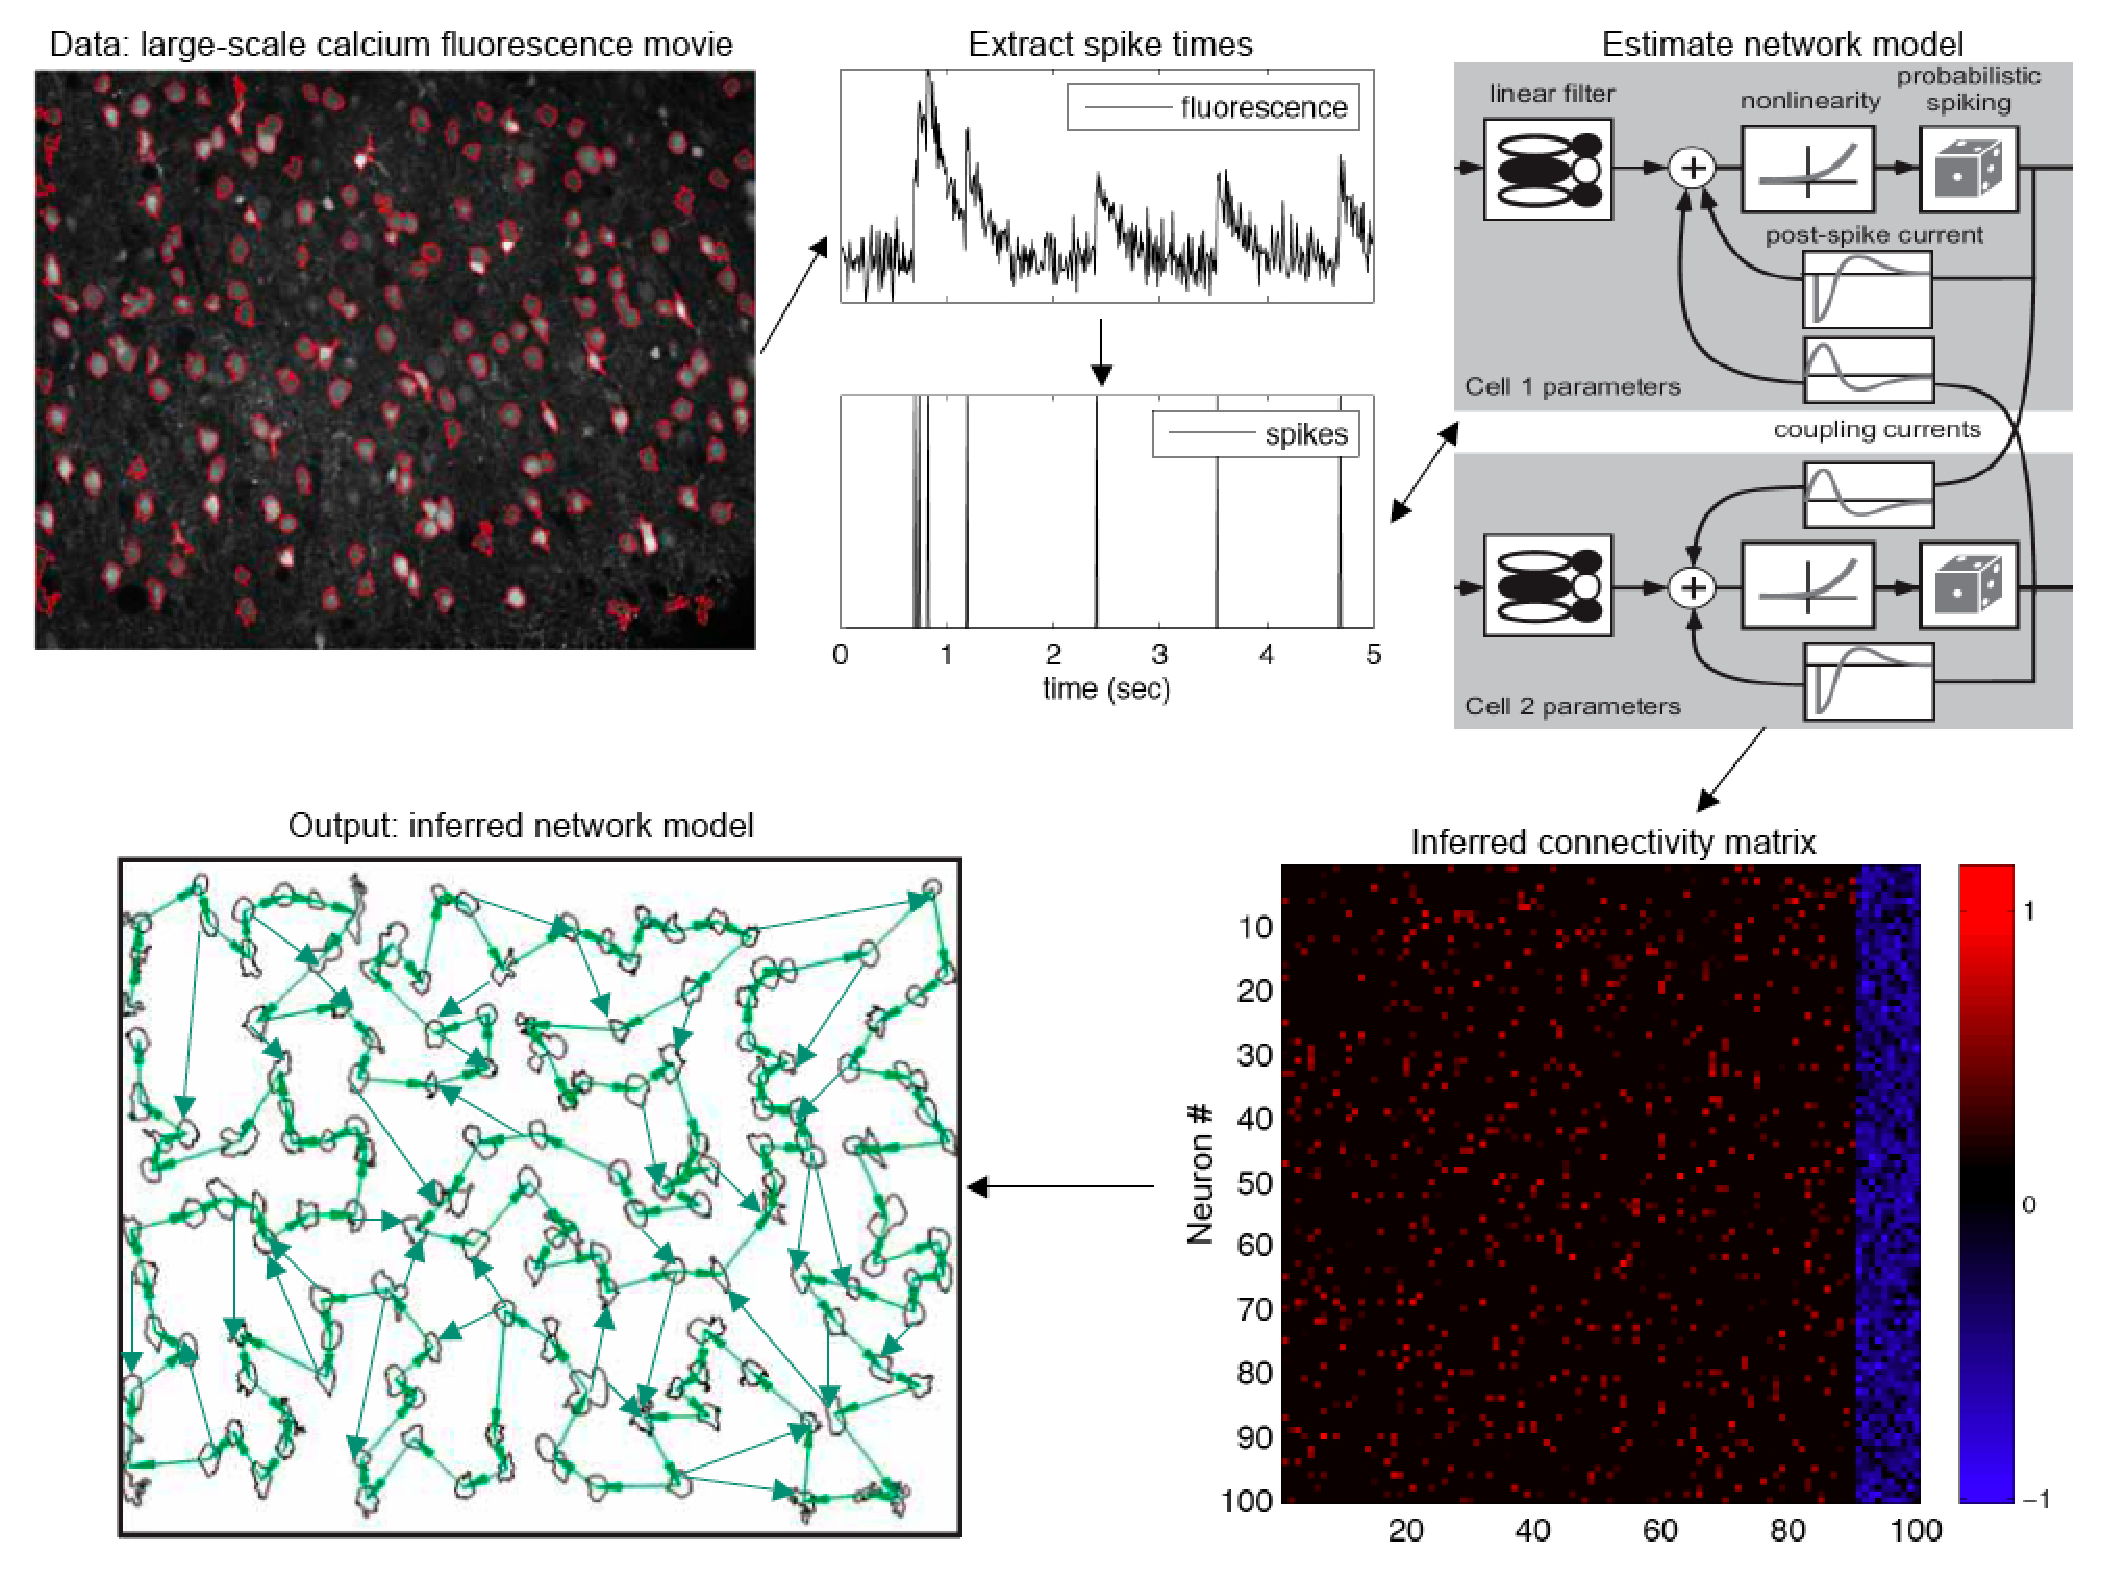
\includegraphics[width=\hsize]{../figs/yuri-paper-schematic}
\caption{Schematic overview. First we obtain large-scale calcium recordings of spontaneous 
and evoked neural responses.  These movies are then pre-processed to correct for movement artifacts, find regions-of-interest, and extract spike trains.  Second, given the fluorescence traces from each neuron, we infer spike trains.  Third, we use our population model to infer the most likely functional connectivity matrix, which is our approximation of the microcircuit.}
\label{fig:data_schematic}
\end{figure}


